\documentclass[a4paper]{article}
\usepackage[spanish]{babel}
\usepackage[utf8]{inputenc}
\usepackage{float}
\usepackage{graphicx}
%\usepackage[american voltage]{circuitikz}
\usepackage{amsmath}
\usepackage{xcolor}
\usepackage{caption}
\usepackage{subcaption}
\usepackage[bottom]{footmisc}


\begin{document}
	\subsection{Introducción}
	Los amplificadores de instrumentación, también conocidos como \textbf{IN-AMP},  son utilizados para amplificar con alta precisión las señales provenientes de diversas unidades de adquisición de datos que no poseen la amplitud suficiente como para poder ser aprovechada siendo muy susceptible a contaminación por ruido . Sin embargo, amplificar no es el único objetivo de este dispositivo. Si así fuese entonces bastaría con utilizar un amplificador operacional corriente.
	\subsubsection{Diferencias entre \textbf{IN-AMP} y \textbf{OP AMP}}
	A simple vista un \textbf{IN-AMP} puede ser fácilmente confundido con un \textbf{OP AMP} dado que tiene varios rasgos en común. En primer lugar ambos dispositivos amplifican una señal diferencial, es decir que multiplican por un cierto factor la diferencia de potencial entre sus terminales de entrada. Por otro lado también poseen una elevada impedancia de entrada (del orden de los Megaohms) y una muy baja impedancia de salida de unos pocos ohms.
	No obstante, podemos notar algunas diferencias fundamentales entre ambos. Por ejemplo, para configurar la ganancia a lazo cerrado de un amplificador operacional se debe ajustar mediante resistores de retro-alimentación externos mientras que en un amplificador de instrumentación la ganancia puede venir predefinida por el fabricante o ajustada mediante una única \textbf{resistencia externa} denominada usualmente como \textbf{$R_{gain}$}.
	En caso de que se desee amplificar una señal diferencial el amplificador de instrumentación eliminara cualquier componente de señal común a ambas entradas como puede ser un offset de continua o simplemente ruido. Esta característica es la que hace especiales a los amplificadores de instrumentación ya que permiten reducir de manera significativa el ruido de las señales recibidas.  
	Por el contrario, los amplificadores operacionales tradicionales que no están diseñados para eliminar este tipo señales no deseadas.

	
	\subsection{Características del IN-AMP}
	El circuito a analizar es una variante de los famosos amplificadores de instrumentación que utilizan 3 amplificadores operacionales que se puede observar en la figura debajo.
	%Imagen del amplificador de instrumentación con 3 op-amps
	\begin{figure}[H]
		\centering
		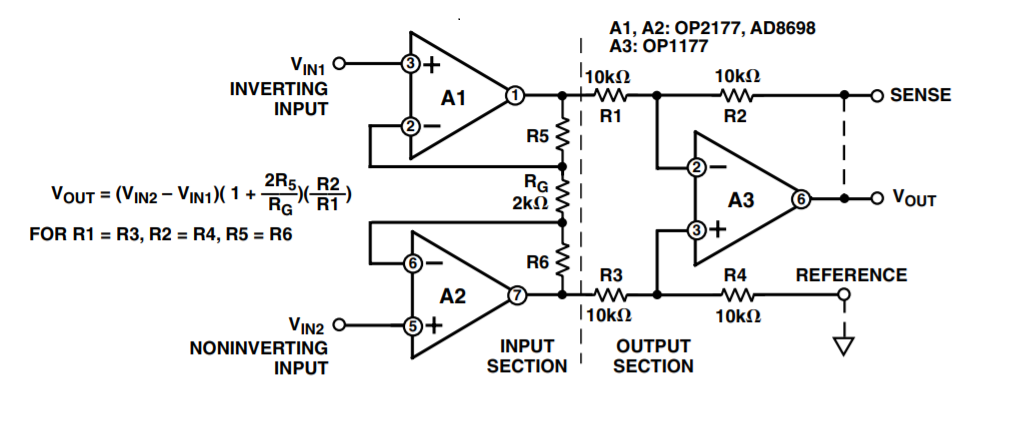
\includegraphics[width=\linewidth]{../ImagenesVarias/inAmp3Opamp}
		%TODO revisar footnote imagen 
		\caption{Clásico amplificador de instrumentación con 3 Opamps}
	\end{figure}
	%\footnote{Imagen extraída de: \textit{A designer's guide to Sinstrumentation amplifiers}
		
	Como se puede apreciar a la izquierda de la línea punteada se han colocado un par de buffers con ganancia. El objetivo de los mismos es de el de aumentar significativamente la impedancia de entrada del in-amp para independizarla lo más posible de la impedancias de las fuentes ya que este pueden ser muy altas o estar desbalanceadas. También ofrece la ventaja de no cargar a la fuente, lo cual es de gran relevancia al trabajar con señales pequeñas. Además le otorga una cierta ganancia a la señal de entrada. Este aspecto del circuito se debe tener en cuenta para evitar la saturación de los op-amps y perder la efectividad del circuito. Analizaremos esta y otras situaciones en secciones posteriores.
	En nuestro caso se trabajara con la versión de 4 amplificadores operacionales.
	
	\begin{figure}[H]
		\centering
		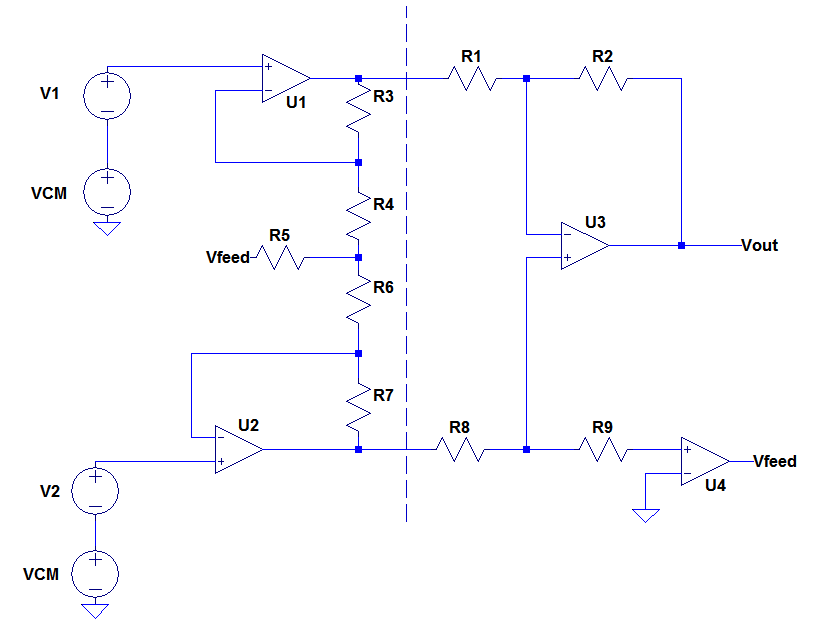
\includegraphics[width=\linewidth]{../ImagenesVarias/inAmpSch.png}
		\caption{Amplificador de instrumentación de 4 op-amps}
	\end{figure}

	Haciendo uso de la herramienta de análisis simbólico \textit{SapWin \footnote{SapWin es una programa de análisis y simulación de circuitos desarrollado por la \textit{Universitá degli studi Firenze}}} obtenemos la siguiente expresión para la ganancia ideal de amplificador de instrumentación:
	\begin{equation}
			V_{out}=\frac{-V_1 R_2 R_4 R_7 - 
			V_1 R_2 R_3 R_7 +
			V_2 R_2 R_3 R_7+
			V_2 R_2 R_3 R_6
		}{R_1 R_4 R_7}
		\label{eqn:idealTrans}
	\end{equation}

	
	Notamos que en la situación ideal tanto las resistencias $R_5$ y $R_9$ no afectan la ganancia del circuito.
	\subsubsection{Relaciones entre los componentes}
	Una de las finalidades del amplificador de instrumentación es la de eliminar aquellas señales que sean comunes a las señales de entrada.
	Por tal motivo comenzaremos por establecer condiciones que nos permitan eliminarlas. 
	Para eso aplicaremos superposición y analizaremos los efectos de $V_{CM}$ sobre la relación anterior.
	
	\begin{figure}[H]
		\centering
		\includegraphics[width=\linewidth]{../ImagenesVarias/inAmpVCM.png}
		\caption{Amplificador de instrumentación de 4 op-amps en modo común}
	\end{figure}
	Obteniendo como transferencia:
	\begin{equation}
		\frac{V_{out}}{V_{CM}}=
		\frac{-R_2 R_4 R_7 - 
			R_2 R_3 R_7 +
			R_2 R_3 R_7+
			R_2 R_3 R_6
		}{R_1 R_4 R_7}
	\end{equation}
		
	Como se quiere que aquellas señales comunes a ambas entrada sean eliminadas pedimos $V_{out}=0$.
	Entonces obtenemos:
		\begin{equation}
		 0=\frac{-V_{CM} R_2 R_4 R_7 - 
				V_{CM} R_2 R_3 R_7 +
				V_{CM} R_2 R_3 R_7+
				V_{CM} R_2 R_3 R_6
			}{R_1 R_4 R_7} 
		\end{equation}
	
	Simplificando
	\begin{equation}
		R_7(R_4+R_3)=R3(R7+R6)
	\end{equation}
	
	\begin{equation}
		R_7R_4+ R_3R_7=R_3R_7+R_3R_6
	\end{equation}
	Cancelando los términos comunes a ambos miembros
	\begin{equation}
		R_7R_4=R_3R_6
	\end{equation}
	Por lo tanto llegamos a:
	\begin{equation}
		\frac{R_4}{R_6}=\frac{R_3}{R_7}  %Relación entre las resistencias de la etapa de amplificación
	\end{equation}

	Aplicando estas relaciones a \eqref{eqn:idealTrans} obtenemos:
	\begin{equation}
		V_{out} = (V_2-V_1)\left[\frac{R_2}{R_1}(1+\frac{R_3}{R_4})\right]
	\end{equation}

\subsection{Generación de señales con puente de Wheatstone}
 	
\begin{thebibliography}{9}
	
	\bibitem{Franco} 
	SERGIO, F. (2002). Design with operational amplifiers and analog integrated circuits. New York [etc.]: McGraw-Hill, pp.73-91.	
	
	\bibitem{Coughlin} 
	R. Coughlin and F. Driscoll, Circuitos integrados lineales y amplificadores operacionales. México: Prentice-Hall Hispanoamericana, 1998.
	
	\bibitem{dguideinamp}
	C. Kitchin and L. Counts, A designer's guide to instrumentation amplifiers. Norwood, Mass.: Analog Devices, 2006.
	
	\bibitem{an244}
	Jeffrey R. Riskin, A User's guide to IC instrumentation amplifiers. Norwood, Mass.: Analog Devices.
	
\end{thebibliography}

\end{document}